\documentclass[11pt,a4paper]{article}
\usepackage[utf8x]{inputenc}
\usepackage{ucs}
\usepackage[spanish]{babel}
\usepackage[left=2cm,top=2cm,right=2cm,bottom=3cm]{geometry} 
\usepackage{amsmath}
\usepackage{amsfonts}
\usepackage{amssymb}
\usepackage{dcolumn}
\usepackage{float}
\usepackage{graphicx}
\usepackage{ esint }
\usepackage{fancyhdr}
\usepackage{enumerate} 
\pagestyle{fancy}
\usepackage{tocbibind}
\usepackage{setspace}
\usepackage{parskip}
\usepackage[hidelinks]{hyperref}
\usepackage{listings} 
\usepackage[svgnames]{xcolor}

\definecolor{codegreen}{rgb}{0,0.6,0}
\definecolor{codegray}{rgb}{0.5,0.5,0.5}
\definecolor{codepurple}{rgb}{0.58,0,0.82}
\definecolor{backcolour}{rgb}{0.95,0.95,0.92}


\definecolor{dkgreen}{rgb}{0,0.6,0}
\definecolor{gray}{rgb}{0.5,0.5,0.5}
\definecolor{mauve}{rgb}{0.58,0,0.82}


\lstset{basicstyle=\ttfamily}
\lstdefinestyle{mystyle}{
	%backgroundcolor=\color{backcolour},   
	commentstyle=\color{codegreen},
	keywordstyle=\color{magenta},
	numberstyle=\tiny\color{codegray},
	stringstyle=\color{codepurple},
	breakatwhitespace=false,         
	breaklines=true,                 
	keepspaces=true,                 
	numbers=left,                    
	%numbersep=5pt                  
}

\lstdefinestyle{customasm}{
  belowcaptionskip=1\baselineskip,
  frame=L,
  xleftmargin=\parindent,
  language= Python,
  basicstyle=\footnotesize\ttfamily,
  commentstyle=\itshape\color{purple!40!black},
}

\lstset{literate=
  {á}{{\'a}}1 {é}{{\'e}}1 {í}{{\'i}}1 {ó}{{\'o}}1 {ú}{{\'u}}1
  {Á}{{\'A}}1 {É}{{\'E}}1 {Í}{{\'I}}1 {Ó}{{\'O}}1 {Ú}{{\'U}}1
  {à}{{\`a}}1 {è}{{\`e}}1 {ì}{{\`i}}1 {ò}{{\`o}}1 {ù}{{\`u}}1
  {À}{{\`A}}1 {È}{{\'E}}1 {Ì}{{\`I}}1 {Ò}{{\`O}}1 {Ù}{{\`U}}1
  {ä}{{\"a}}1 {ë}{{\"e}}1 {ï}{{\"i}}1 {ö}{{\"o}}1 {ü}{{\"u}}1
  {Ä}{{\"A}}1 {Ë}{{\"E}}1 {Ï}{{\"I}}1 {Ö}{{\"O}}1 {Ü}{{\"U}}1
  {â}{{\^a}}1 {ê}{{\^e}}1 {î}{{\^i}}1 {ô}{{\^o}}1 {û}{{\^u}}1
  {Â}{{\^A}}1 {Ê}{{\^E}}1 {Î}{{\^I}}1 {Ô}{{\^O}}1 {Û}{{\^U}}1
  {œ}{{\oe}}1 {Œ}{{\OE}}1 {æ}{{\ae}}1 {Æ}{{\AE}}1 {ß}{{\ss}}1
  {ű}{{\H{u}}}1 {Ű}{{\H{U}}}1 {ő}{{\H{o}}}1 {Ő}{{\H{O}}}1
  {ç}{{\c c}}1 {Ç}{{\c C}}1 {ø}{{\o}}1 {å}{{\r a}}1 {Å}{{\r A}}1
  {€}{{\euro}}1 {£}{{\pounds}}1 {«}{{\guillemotleft}}1
  {»}{{\guillemotright}}1 {ñ}{{\~n}}1 {Ñ}{{\~N}}1 {¿}{{?`}}1
}

\lstset{showstringspaces=false}
\lstloadlanguages{Python}
\lstset{basicstyle=\ttfamily\footnotesize}
\lstset{style=mystyle}
\usepackage[titletoc,toc,page]{appendix}
\usepackage{pdfpages}
\renewcommand{\appendixtocname}{Anexo}
\renewcommand{\appendixpagename}{Anexo}
\lhead{ Modelos y Simulación- TP1 }
\rhead{
\includegraphics[width=1.5 cm]{imagenes/logo}}
\author{cyn}
\begin{document}
\begin{titlepage}
\begin{center}
\vspace*{-1in}
\begin{figure}[htb]
\begin{flushleft}

\includegraphics[width=5cm]{imagenes/logo}
\end{flushleft}
\end{figure}
\begin{LARGE}
\textbf{U.B.A. FACULTAD DE INGENIERÍA}\\
\end{LARGE}
\vspace*{0.15in}
\begin{LARGE}
\textbf{Departamento de Computación}\\
\end{LARGE}
\vspace*{0.2in}
\begin{LARGE}
\textbf{Modelos y Simulación 7526 - 9519}\\
\end{LARGE}
\vspace*{0.2in}
\begin{Large}
\textbf{TRABAJO PRÁCTICO \#1}\\
\end{Large}
\vspace*{0.2in}
\begin{LARGE}
\textit{Números al azar y Test estadísticos }\\
\end{LARGE}
\vspace*{0.2in}
\begin{Large}
\raggedright\textbf{Curso: 2019 - 1er Cuatrimestre}\\
\end{Large}
\vspace*{0.1in}
\begin{Large}
\raggedright\textbf{Turno: Miércoles}\\
\end{Large}
\vspace*{0.1in}

\begin{table}[htb]
\begin{center}
\begin{spacing}{1.9}
\begin{tabular}{| l | l |}
\hline
\multicolumn{2}{|>{\arraybackslash}p{15cm}|}{\begin{Large}
\textbf{GRUPO N° 1}
\end{Large}}\\
\hline
\textbf{Integrantes} & \textbf{Padrón} \\
\hline
\makebox[8cm][c]{Amurrio, Gastón} & \makebox[2.5cm][c]{93584}\\
\hline
\makebox[8cm][c]{Gamarra Silva, Cynthia Marlene} & \makebox[2.5cm][c]{92702}\\
\hline
\makebox[8cm][c]{Pinto, Tomás} & \makebox[2.5cm][c]{98757}\\
\hline
\textbf{Fecha de Entrega: } & \hspace{0.8cm}24-04-2019\\
\hline
\textbf{Fecha de aprobación: } & \\
\hline
\textbf{Calificación: } & \\
\hline
\textbf{Firma de aprobación:} & \\
\hline
\end{tabular}
\end{spacing}
\end{center}
\end{table}
\fbox{%
\begin{minipage}[c][3.4cm][l]{.9\linewidth}
\textbf{Observaciones:} \\
\vfill
\end{minipage}
}
\end{center}

\vspace*{0.1in}
\end{titlepage}
\tableofcontents 
\vspace*{0.3in}
\newpage

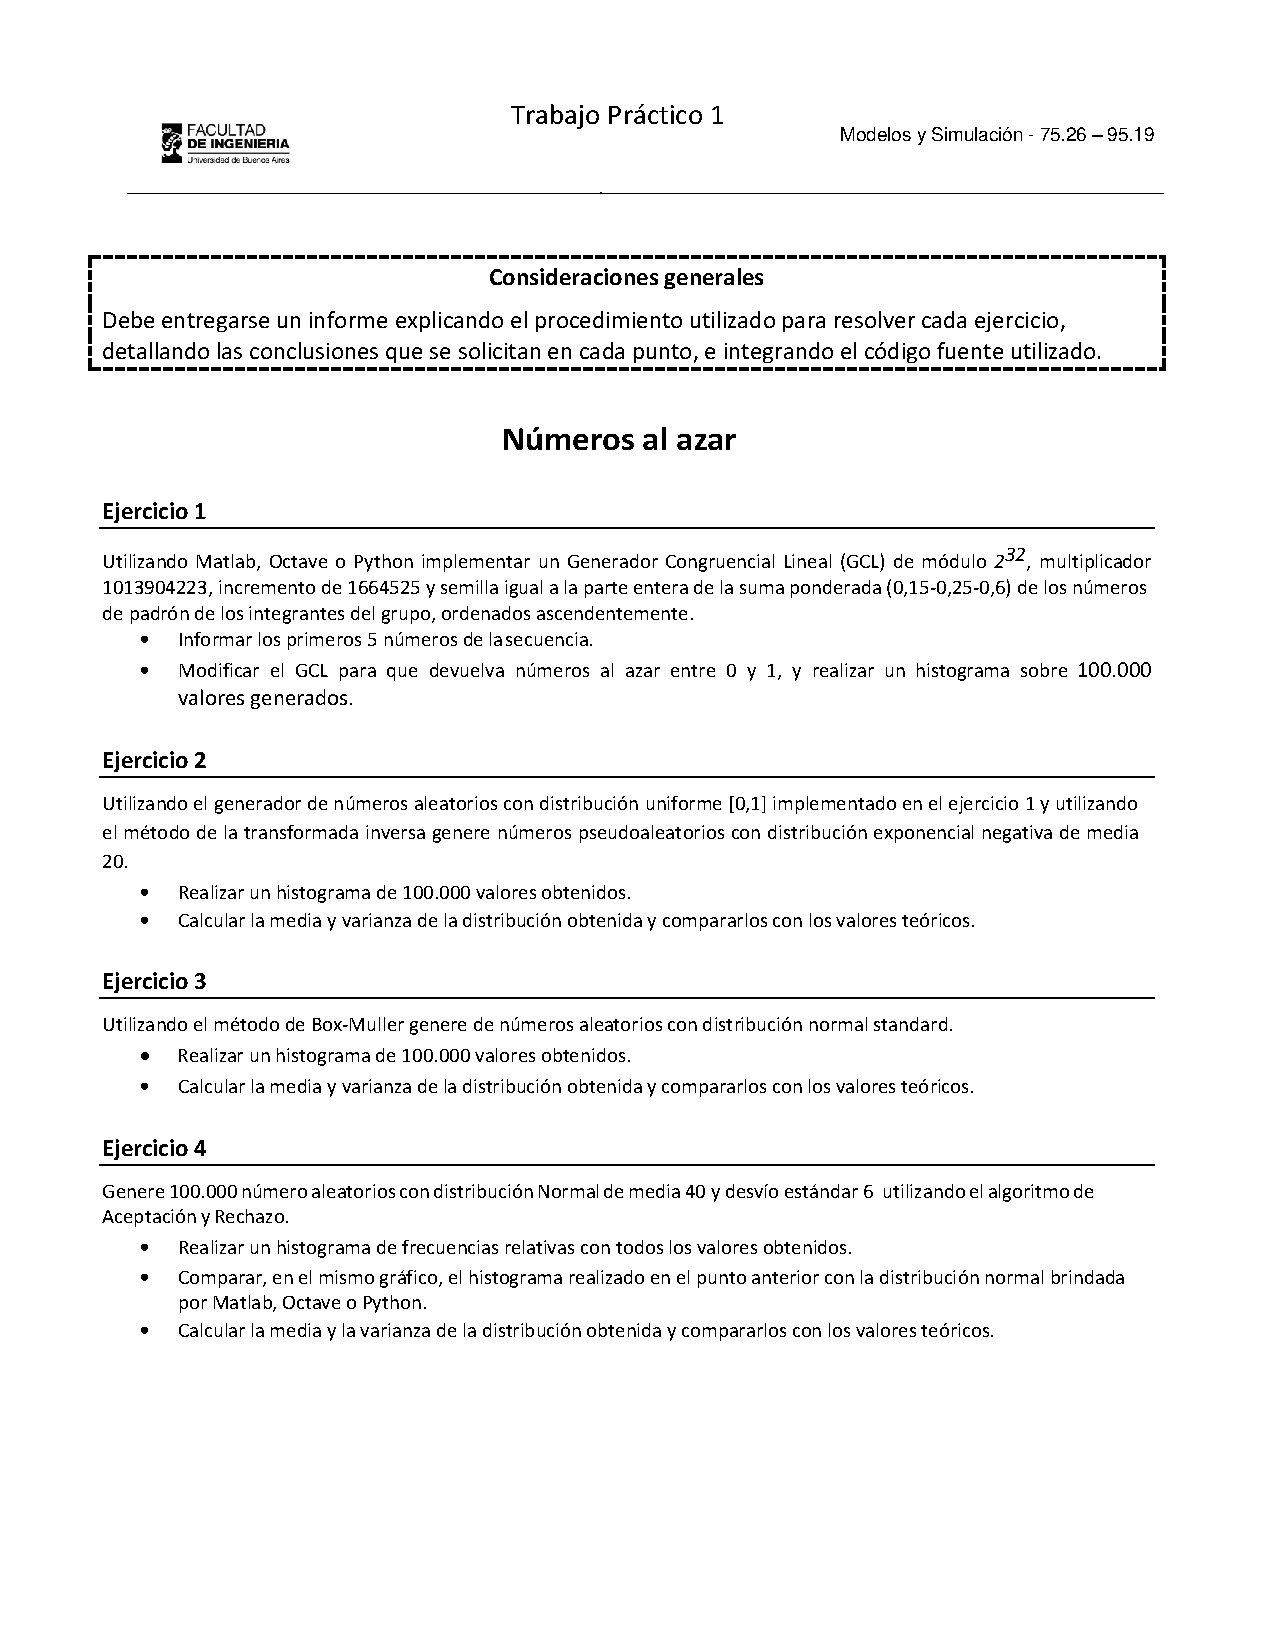
\includepdf[pages=1,scale=0.95,pagecommand = \section{Enunciado del trabajo práctico}\label{enunciado},offset=10 -10]{FIUBA-Simulacion-TrabajoPractico1.pdf}
\includepdf[pages={2-last},scale=0.95,pagecommand = {},offset=10 -10]{FIUBA-Simulacion-TrabajoPractico1.pdf}


\newpage

\section{Introducción}
El trabajo práctico consiste en aplicar conceptos teóricos explicados en clase sobre generación de números aleatorios aplicado a distintos métodos estadísticos utilizados en el medio ciéntifico como ser Box Muller, Generador Congruencial Lineal (GCL), Tranformada inversa y tests como Test espectral y Kolmogorov-Smirnov.
Los ejercicios están simulados en lenguaje Python.

\section{Implementación y resultados}
Para cada uno de los ejercicios pedidos se realiza una explicación de cada uno de ellos. Se toma como base teórica lo explicado en clase tanto teórica como clase práctica.

	\subsection{Ejercicio 1}
	    Para realizar el ejercicio aplicamos lo siguiente:
	    \begin{enumerate}
	        \item Creamos la secuencia de números utilizando una Generador Congruencial Lineal( GCL ). Los datos utilizados para el GCL son:
	            \begin{itemize}
	                \item módulo = $2^{32}$
	                \item multiplicador = 1013904223
	                \item incremento = 1664525
	                \item semilla = $92702*0.15+93584*0.25+98757*0.26$
	            \end{itemize}
	         \item Para que de números entre 0 y 1 se divide por su módulo
	         \item Graficamos el histograma utilizando la secuencia creada.
	         
	    \end{enumerate}
		El resultado de los primeros 5 números de la secuencia: [62978, 383030987L, 2740587618L, 1650525291L, 2470812354L].\\
		El histograma pedido utilizando el método Generador Congruencial Lineal (GCL) donde se grafica para números al azar entre 0 y 1,es el siguiente:
		\begin{figure}[H]
  			\centering
    			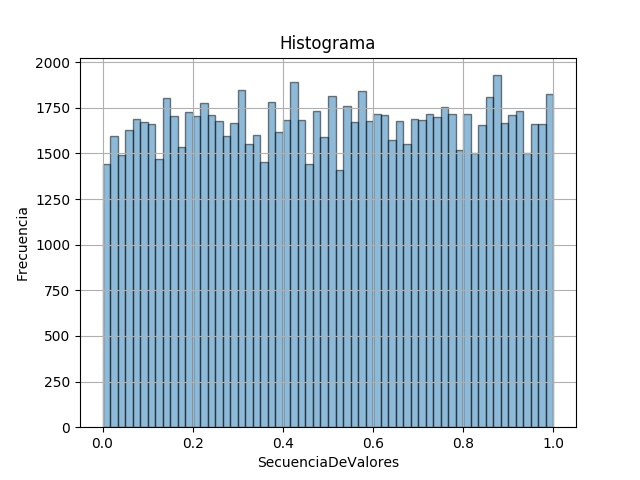
\includegraphics[width=11cm]{imagenes/histogramaEjer1}
		\end{figure}

	\subsection{Ejercicio 2}
	    Para realizar el ejercicio aplicamos lo siguiente:
	    \begin{enumerate}
	        \item Creamos la secuencia utilizando GCL con los mismos datos del ejercicio anterior.
	        \item A la secuencia creada le dividimos por su módulo para obtener números entre 0 y 1.
	        \item Aplicamos la función transformada inversa a la secuencia.
	        \item Realizamos un histograma con la nueva secuencia.
	        \item Calculamos la media y varianza de la distribución simulada y teórica.
	    \end{enumerate}
	    
		El histograma pedido utilizando el método de la transformada inversa generado con números pseudoaleatorios con distribución exponencial negativa de media 20 es el siguiente:
		\begin{figure}[H]
  			\centering
    			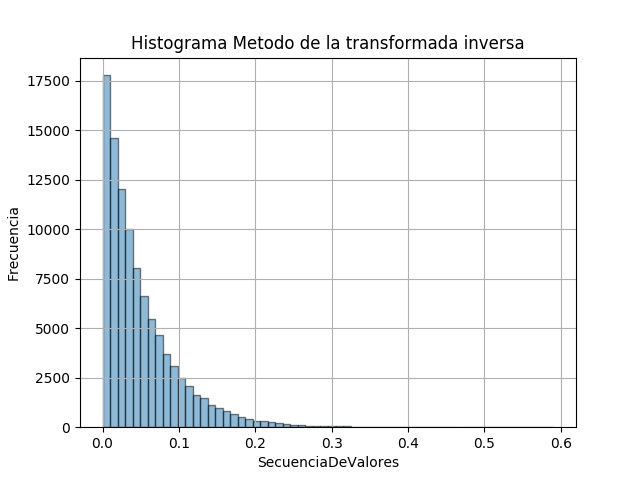
\includegraphics[width=12cm]{imagenes/histogramaEjer2}
		\end{figure}
		Comparando los resultados simulados y teóricos:
		\begin{itemize}
			\item El valor simulado de la media es 0.0501097366318
			\item El valor teórico de la media es 0.05
			\item El valor simulado de la varianza es 0.00250751904958
			\item El valor teórico de la varianza es 0.0025
		\end{itemize}
		
		Por lo tanto podemos observar que los valores simulados y teóricos son bastantes parecidos.

	\subsection{Ejercicio 3}
	    Para realizar el ejercicio aplicamos lo siguiente:
	    \begin{enumerate}
	        \item Creamos dos listas: u1 y u2 con valores de distribución normal 0, 1.
	        \item Aplicamos el método de Box Muller a estas dos listas y obtenemos dos listas nuevas z1 y z2.
	        \item Realizamos histogramas con z1 y z2 y otro histograma con una distribución normal estándar.
	        \item Calculamos la media y varianza de la distribución simulada y teórica.
	    \end{enumerate}

		Los resultados que obtenemos son los siguientes:
		\begin{itemize}
			\item El valor simulado de la media z1 es 0.000743926097041
			\item El valor simulado de la media z2 es -0.0016462929471
			\item El valor teórico de la media es 0 
			\item El valor simulado de la varianza z1 es 0.998271254875
			\item El valor simulado de la varianza z2 es 0.996519878651
			\item El valor teórico de la varianza es 1
		\end{itemize}

		El histograma pedido utilizando Box Muller es el siguiente:
		\begin{figure}[H]
  			\centering
    			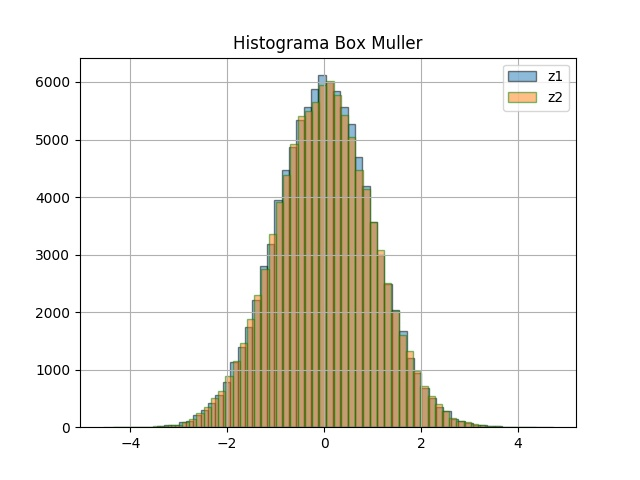
\includegraphics[width=14cm]{imagenes/histogramaEjer3}
		\end{figure}

		Si comparamos con una distribución Normal estándar obtenemos:
		\begin{figure}[H]
  			\centering
    			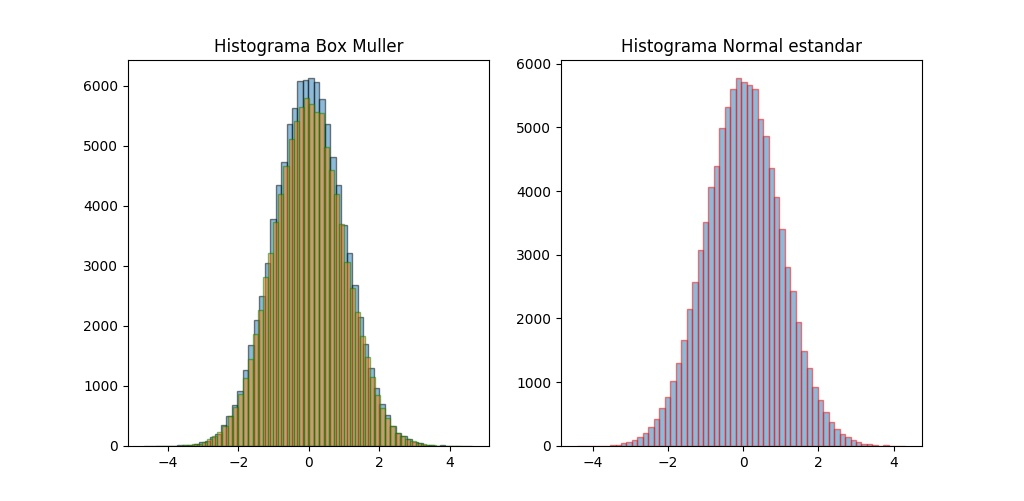
\includegraphics[width=20cm]{imagenes/histogramasEjer3}
		\end{figure}
		
		Por lo tanto podemos observar que se comprueba que el método de Box Muller es una distribución normal estándar.



	\subsection{Ejercicio 4}

	Seguimos los pasos de esta guia: \href{https://wiseodd.github.io/techblog/2015/10/21/rejection-sampling/}{ Rejection Sampling}.

	La distribucion target $P(x)$ es una $N(40,6)$
	\begin{figure}[H]
  			\centering
    			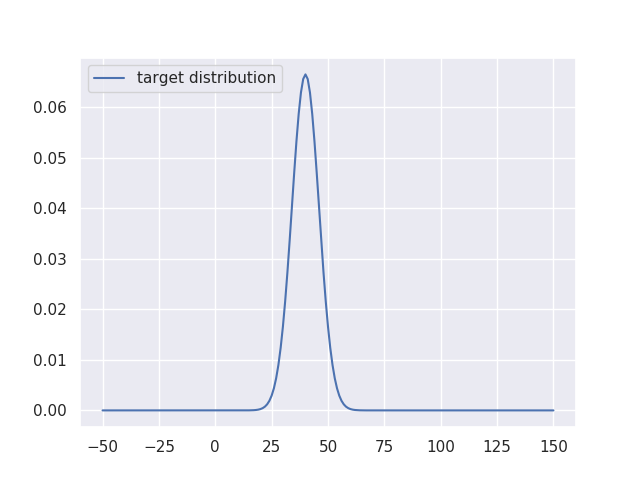
\includegraphics[width=14cm]{imagenes/target}
	\end{figure}

	Proponemos $Exp(0.01)$ como $Q(x)$
	\begin{figure}[H]
  			\centering
    			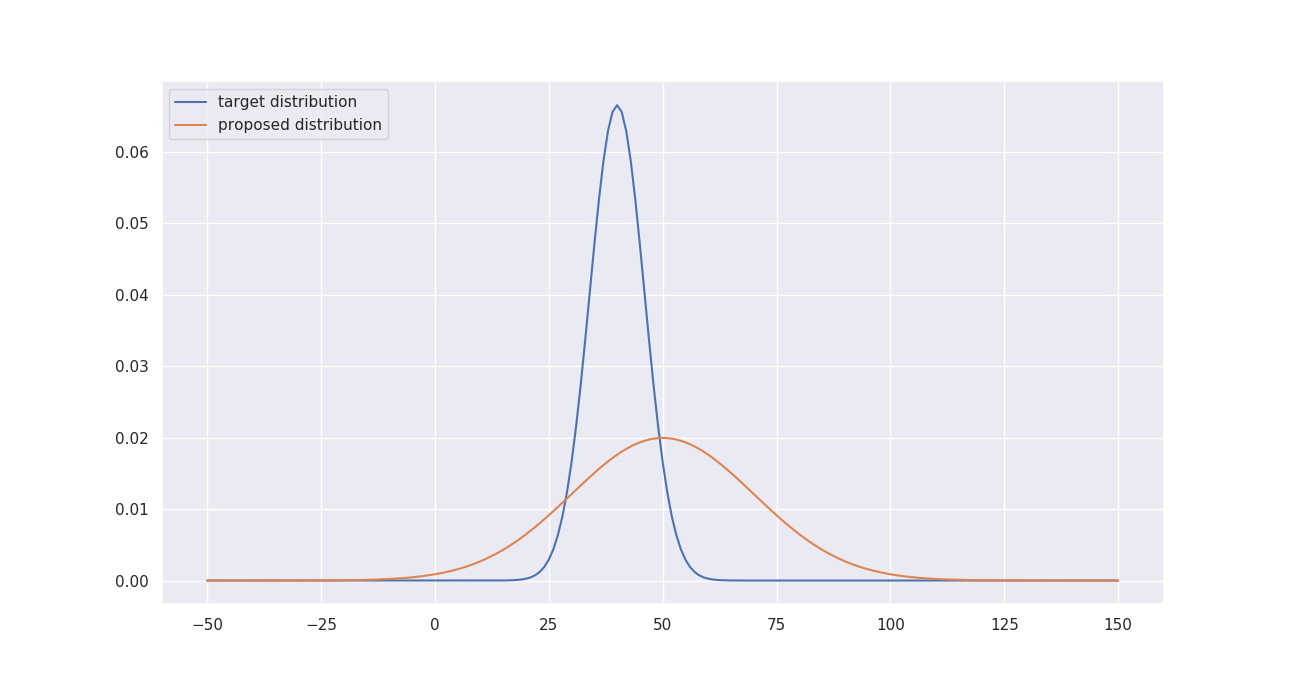
\includegraphics[width=14cm]{imagenes/proposed}
	\end{figure}
	Rejection Sampling va a fallar debido a que la $Q(x)$ propuesta no esta envolviendo a nuestra distribucion target $P(x)$
	\begin{figure}[H]
  			\centering
    			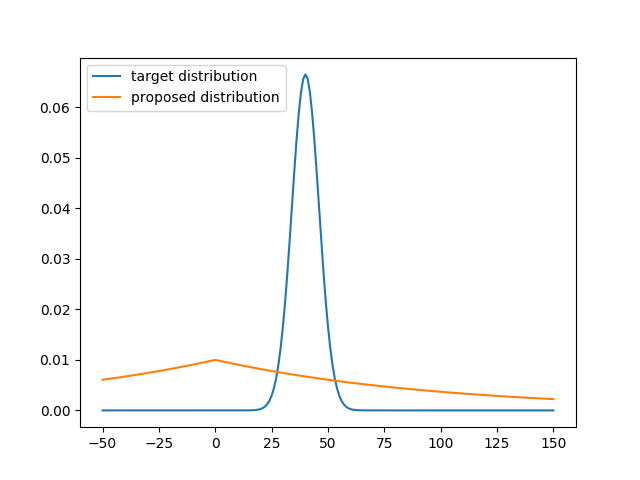
\includegraphics[width=14cm]{imagenes/proposed_not_escaled}
	\end{figure}
	Para remediar esto, encontramos un factor k que multiplique a $Q(x)$ que es la relacion maxima entre $P(x)$ y $Q(x)$, entonces:
	\begin{align*}
		k = max(P(x) / Q(x)) for all x
	\end{align*}

	Al reescalar..
	\begin{figure}[H]
  			\centering
    			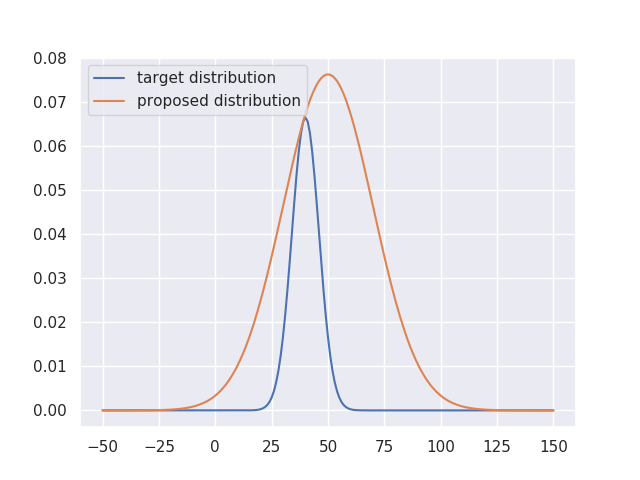
\includegraphics[width=18cm]{imagenes/proposed_escaled}
	\end{figure}

	La distribucion generada mediante rejection sampling es la siguiente:
	\begin{figure}[H]
  			\centering
    			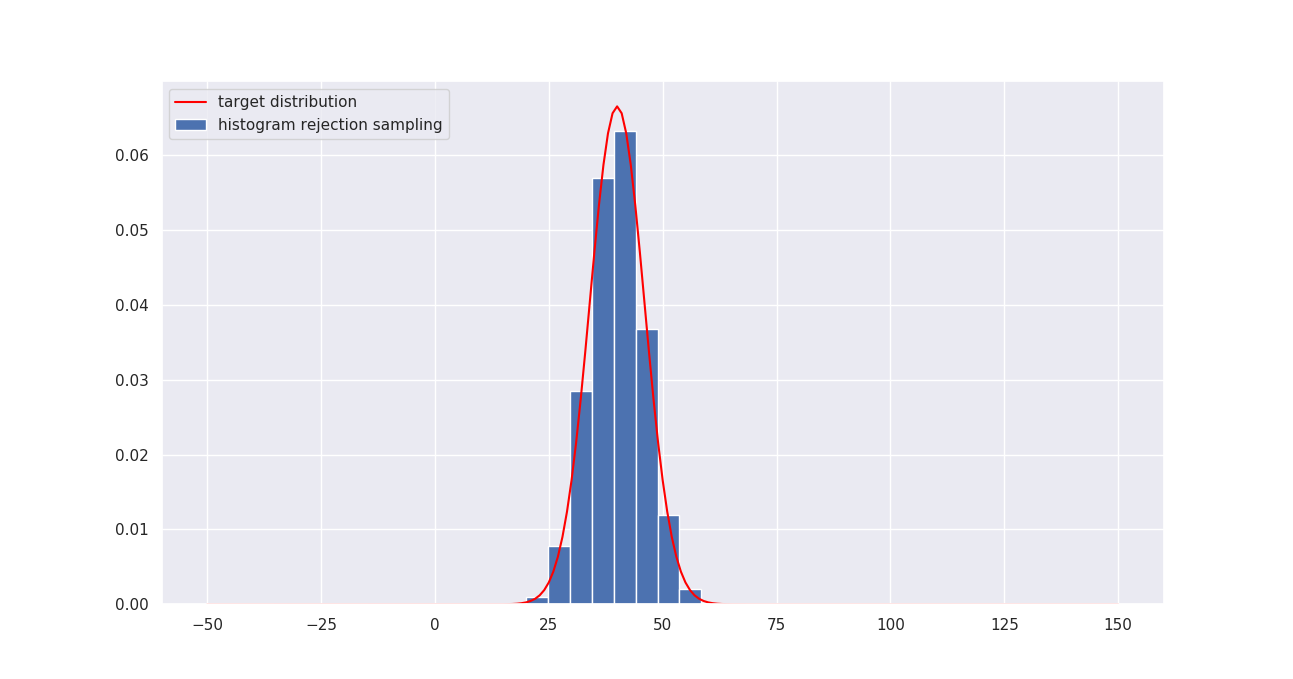
\includegraphics[width=14cm]{imagenes/rejection_sampling_generated_distribution}
	\end{figure}

	Este es el grafico de la distribucion real vs el histograma de valores generados por el algoritmo. 
	Como podemos ver, el algoritmo logro generar una aproximacion bastante buena. 

	La media de la muestra generada se encuentra alrededor de 40, y la varianza cerca de 36.\newline
	La varianza muestral es mucho mas amplia comparada con la teorica. La media muestral es la misma.

	\subsection{Ejercicio 5}
	    Para realizar el ejercicio aplicamos lo siguiente:
	    \begin{enumerate}
	        \item Se genera 100000 valores utilizando GCL.
	        \item A la secuencia creada le dividimos por su módulo para obtener números entre 0 y 1.
	        \item Aplicamos la función transformada inversa a la secuencia utilizando la función de distribución de probabilidad empírica.
	        \item Realizamos un histograma con la nueva secuencia.
	    \end{enumerate}
	
		El histograma pedido utilizando la función de distribución de probabilidad empírica dada por el enunciado:
		\begin{figure}[H]
  			\centering
    			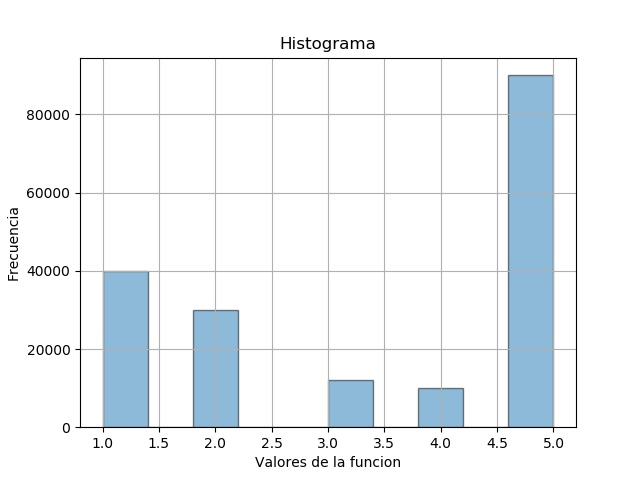
\includegraphics[width=14cm]{imagenes/histogramaEjer5}
		\end{figure}

	\subsection{Ejercicio 6}
	    Para realizar el ejercicio aplicamos lo siguiente:
	    \begin{enumerate}
	        \item Se genera 2 listas x,y con números aleatorios que provee PYTHON.
	        \item Con ambas listas x,y creamos dos listas nuevas filtrando con aquellas que cumplen $x^2+y^2<1$.
	        \item Realizamos un gráfico utlizando estas dos listas nuevas.
	        
		El gráfico pedido utilizando tilizando una distribucion uniforme entre [-1,1] generado con números aleatorios en un círculo de radio 1 centrado en el origen.
		\end{enumerate}
		\begin{figure}[H]
  			\centering
    			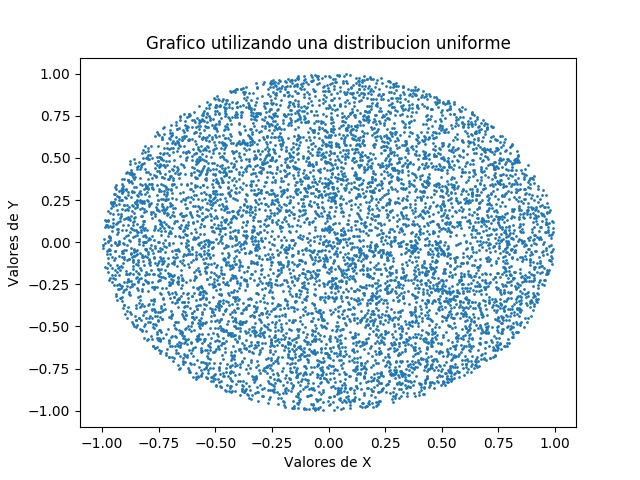
\includegraphics[width=14cm]{imagenes/histogramaEjer6}
		\end{figure}

	\subsection{Ejercicio 7}
        	Para realizar el ejercicio aplicamos lo siguiente:
	    \begin{enumerate}
	        \item Se genera 3 listas x,y,z utilizando el generador GCL.
	        \item Con las listas x,y,z creamos 3 listas nuevas filtrando con aquellas que cumplen:
		\begin{itemize}
			\item GCL($i$),GCL($i+3$),GCL($i+6$),....
			\item GCL($i+1$),GCL($i+4$),GCL($i+7$),....
			\item GCL($i+2$),GCL($i+5$),GCL($i+8$),....
		\end{itemize}


	        \item Realizamos un gráfico utlizando estas dos listas nuevas.
	        
		
	   \end{enumerate}
		El gráfico en 2D es 
		\begin{figure}[H]
  			\centering
    			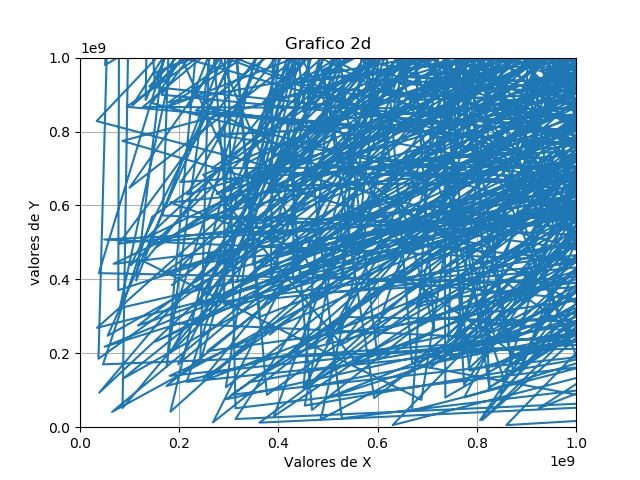
\includegraphics[width=14cm]{imagenes/histogramaEjer72d}
		\end{figure}

		El grafico en 3D es:
		\begin{figure}[H]
  			\centering
    			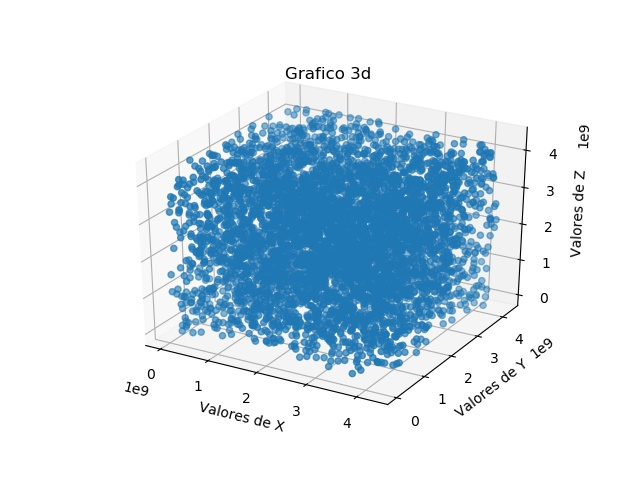
\includegraphics[width=14cm]{imagenes/histogramaEjer73d}
		\end{figure}

	\subsection{Ejercicio 8}
	Utilizando el test Estadístico $Chi^2$ se aplica el método utilizando los siguientes pasos:
	\begin{enumerate}
		\item Utilizamos la distribución empírica generada en el ejercicio 5). Está distribución se corresponderá a $N_i$ ocurrencias observadas.
		\item Obtenemos una distribución uniforme con n = 100.000 muestras generadas
		\item Medimos la dispersion de las ocurrencias obervadas $N_i$ respectos de las esperadas $n*p_i$. La dispersión se calcula como:
		\begin{align*}
		D^2 = \Sigma_{k=1}^{k-1} \frac{(N_i - np_i)^2}{np_i}
		\end{align*}
		\item Calculamos $D^2 < t$ para saber si aceptamos la hipótesis  con un error del 1\%
		
		En nuestro caso obtuvimos que se rechaza la hipótesis con la distribución empirica con un error del 1 \%
	\end{enumerate}

	\subsection{Ejercicio 9}
	Se siguieron los pasos del algoritmo explicado en The Art of Computing Program Volumen 2 de D.E.Knuth, página 62

	Realizamos un grafico para comparar las frecuencias de gaps obtenidas y las esperadas:
	\begin{figure}[H]
  		\centering
    		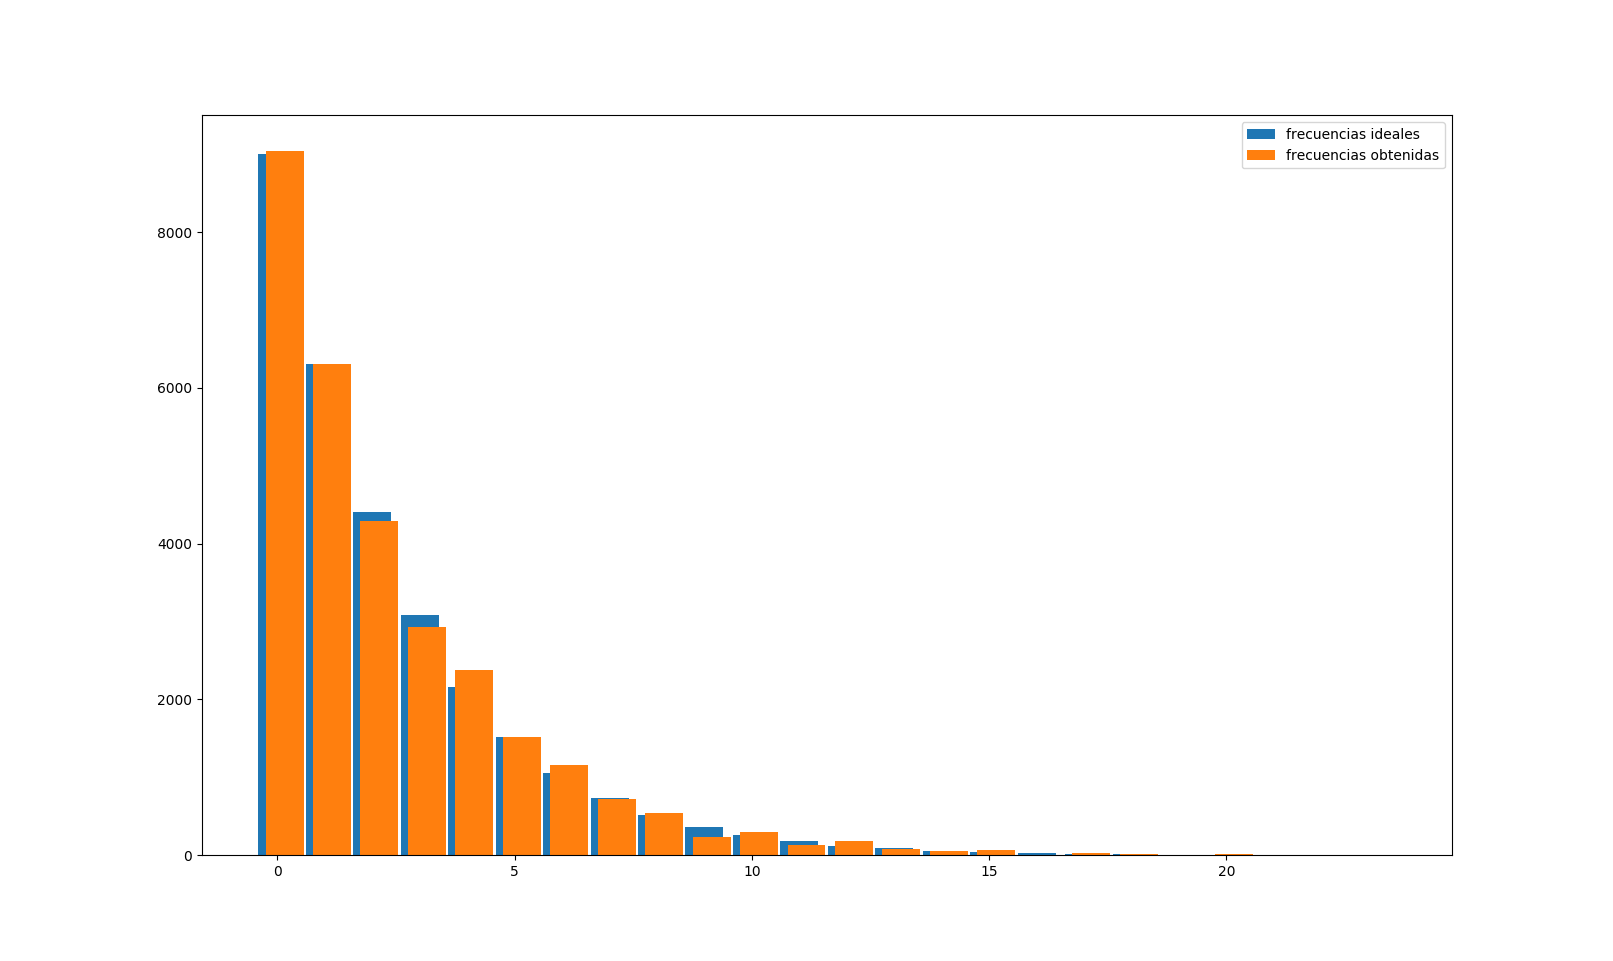
\includegraphics[width=14cm]{imagenes/ej9}
	\end{figure}
	
	Graficamente se espera que pase el test, y asi sucedio con un nivel de significacion 0.05
	\subsection{Ejercicio 10}
	\begin{enumerate}
		\item Nos apoyamos en scipy.stats, especificamente con la clase kstest
		\item Asumimos un nivel de significancia del $0.05$\%
		\item Ambas muestras pasaron el test de kolmogorov-smirnov
	\end{enumerate}
	\begin{figure}[H]
  		\centering
    		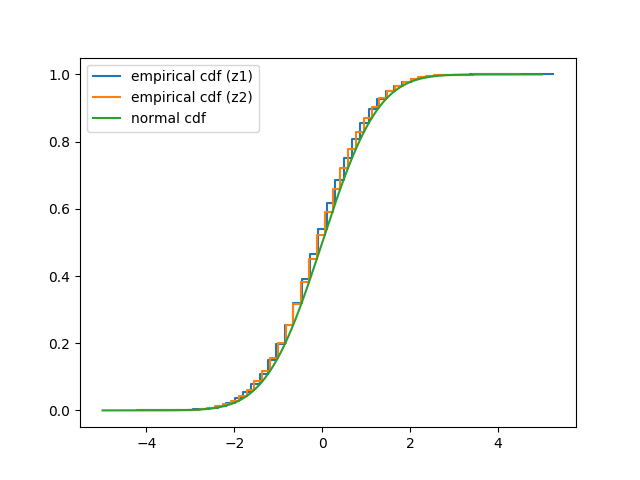
\includegraphics[width=14cm]{imagenes/10}
	\end{figure}
	Como podemos observar mediante las distribuciones empiricas, estas dos variables generadas mediante el metodo Box-Muller se aproximan bastante a una normal real.

\newpage
\section{Conclusiones y aclaraciones}
El trabajo práctico nos permitió conocer y realizar simulaciones teniendo como base teórica los conceptos explicados en clase . Además, nos permitió conocer herramientas que permiten realizar simulaciones qure son muy utilizadas en el campo científico.

En el ejercicio 3 y 10 si bien podriamos haber trabajado con una unica distribucion generada por el metodo, nos parecio interesante trabajar con ambas ya que son generadas de maneras distintas.
\begin{thebibliography}{10}
	\bibitem{} Python, Generación de números con distintas distribuciones de probabilidad, https://docs.python.org/3/library/random.html.
	\bibitem{} Método de Box Muller, https://es.wikipedia.org/wiki/Método\_de\_Box-Muller.
	\bibitem{} Probability, Statistics, and Random Processes for Electrical Engineerging,3rd\_Ed. Leon-Garcia
	\bibitem{} Graficar en python, https://matplotlib.org/api/\_as\_gen/mpl\_toolkits.mplot3d.axes3d.Axes3D.html
\end{thebibliography}


\newpage
%-----------------------------------%
%									%
%			Seccion:Fuente			%
%									%
%-----------------------------------%
\appendix
\section{Código fuente}\label{appendix_codigo_fuente}

	\subsection{Resolución ejercicio 1}\label{ejercicio_1}
		\lstinputlisting[language=Python]{../ejercicios/TPEj1.py}

	\newpage

	\subsection{Resolución ejercicio 2}\label{ejercicio_2}
		\lstinputlisting[language=Python]{../ejercicios/TPEj2.py}

	\newpage

	\subsection{Resolución ejercicio 3}\label{ejercicio_3}
		\lstinputlisting[language=Python]{../ejercicios/TPEj3.py}

	\newpage

	\subsection{Resolución ejercicio 4}\label{ejercicio_4}
		\lstinputlisting[language=Python]{../ejercicios/TPEj4.py}

	\newpage

	\subsection{Resolución ejercicio 5}\label{ejercicio_5}
		\lstinputlisting[language=Python]{../ejercicios/TPEj5.py}

	\newpage

	\subsection{Resolución ejercicio 6}\label{ejercicio_6}
		\lstinputlisting[language=Python]{../ejercicios/TPEj6.py}

	\newpage

	\subsection{Resolución ejercicio 7}\label{ejercicio_7}
		\lstinputlisting[language=Python]{../ejercicios/TPEj7.py}

	\newpage

	\subsection{Resolución ejercicio 8}\label{ejercicio_8}
		\lstinputlisting[language=Python]{../ejercicios/TPEj8.py}

	\newpage

	\subsection{Resolución ejercicio 9}\label{ejercicio_9}
		\lstinputlisting[language=Python]{../ejercicios/TPEj9.py}

	\newpage

	\subsection{Resolución ejercicio 10}\label{ejercicio_10}
		\lstinputlisting[language=Python]{../ejercicios/TPEj10.py}

\end{document}
